\newpage
\begin{homeworkProblem}
    A thick spherical shell carries charge density 
    $$
    \rho = 
    \begin{cases} 
        \frac{k}{r^2}, & \text{for } a \leq r \leq b \\
        0, & \text{otherwise}
    \end{cases}
    $$
    where $k$ is constant. Find the electric field everywhere (for $r < a$, $a < r < b$, and $r > b$). Plot $|E|$ as a function of $r$ for the case of $b = 2a$. In the limit $r \gg b$, does the electric field make sense?
    \begin{callout}{Solution:}

        $$ \nabla \cdot \mathbf{E} = \frac{\rho}{\epsilon_0} $$
        This is the differential form of Gauss's law. It asserts that the divergence of the electric field at any point is proportional to the charge density at that point.

        In its integral form, it is written as
        $$ \oint_{\mathcal{S}} \mathbf{E} \cdot d \mathbf{a} = \frac{Q_{\text{enc}}}{\epsilon_0}, $$
        where the total electric flux through a closed surface \( \mathcal{S} \) equals the enclosed charge \( Q_{\text{enc}} \) divided by \( \epsilon_0 \).

        We now compute the enclosed charge \( Q_{\text{enc}} \) by integrating the charge density over the volume:
        $$ Q_{\text{enc}} = \int_{a}^{r} \frac{k}{r'^2} dV. $$

        The volume element in spherical coordinates is
        $$ dV = r'^2 \sin\phi \, dr' \, d\theta \, d\phi. $$
        For the surface integral, the area element at a fixed radius \( r \) is
        $$ d\mathbf{a} = r^2 \sin\phi \, d\theta \, d\phi. $$

        \begin{enumerate}[i.]
            \item Within the empty space of the closed shell $(r<a)$, there is no enclosed charge
            \item Within the solid section of the shell $(a<r<b)$:
                $$ E r^2 \cancel{\int_{0}^{2\pi} d\theta \int_{0}^{\pi} \sin\phi \, d\phi} = \frac{1}{\epsilon_0} \int_{a}^{r} \frac{k}{\cancel{r'^2}} \cancel{r'^2} dr' \cancel{\int_{0}^{2\pi} d\theta \int_{0}^{\pi} \sin\phi \, d\phi}. $$
                This simplifies to
                $$ E r^2 = \frac{k}{\epsilon_0} (r - a), $$
                and solving for \( E \),
                $$ E = \frac{k(r - a)}{r^2 \epsilon_0}. $$
            \item Outside the shell (r>b), simply set $r\to b$ in the right hand integral:
                $$ E = \frac{k(b - a)}{r^2 \epsilon_0}. $$
        \end{enumerate}

        Finally, when $r \gg b$, the electric field is very close to that of a point charge.

    \end{callout}

    \begin{figure}[ht]
    \centering
    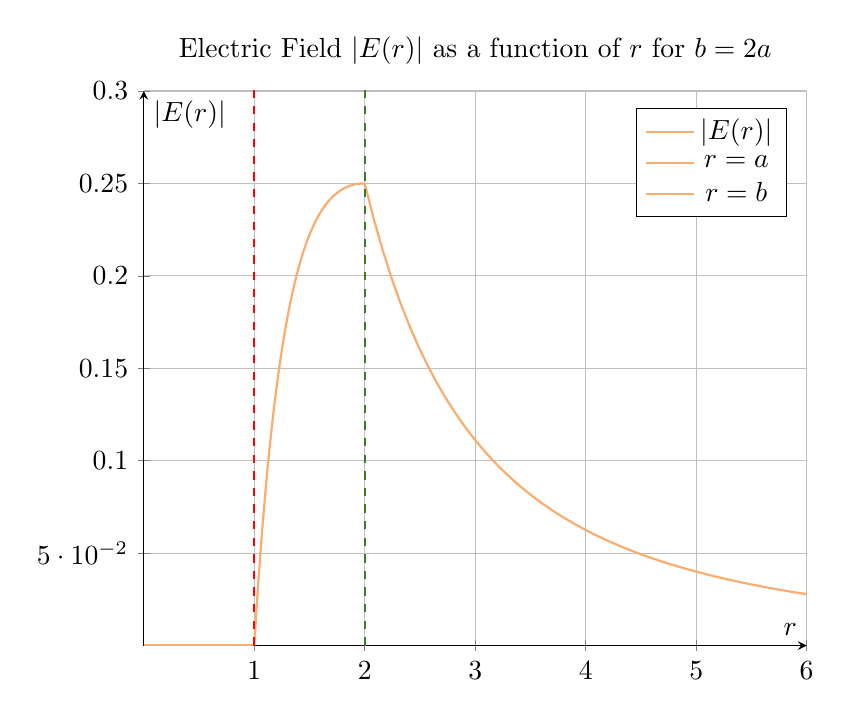
\begin{tikzpicture}
    \begin{axis}[
        width=10cm,
        xlabel={$r$},
        ylabel={$|E(r)|$},
        title={Electric Field $|E(r)|$ as a function of $r$ for $b = 2a$},
        grid=major,
        legend pos=north east,
        axis lines=middle,
        domain=0:6,
        samples=200,
        ymax=1.5,
        xmin=0,
        ymax=0.3
    ]
    
    % Region 1: E(r) = 0 for r < a
    \addplot[domain=0:1, samples=50, thick, Apricot] {0};

    % Region 2: E(r) for a <= r <= b
    \addplot[domain=1:2, samples=50, thick, Apricot] {(x-1)/x^2};
    
    % Region 3: E(r) for r > b
    \addplot[domain=2:6, samples=50, thick, Apricot] {(2-1)/x^2};

    % Mark a and b
    \addplot[dashed, thick, Red] coordinates {(1,0) (1,1)};
    \addplot[dashed, thick, OliveGreen] coordinates {(2,0) (2,1)};
    
    % Annotations for a and b
    \node at (axis cs:1,1.1) [anchor=south east] {$r = a$};
    \node at (axis cs:2,1.1) [anchor=south west] {$r = b$};

    \legend{$|E(r)|$, $r = a$, $r = b$}
    \end{axis}
    \end{tikzpicture}
\end{figure}

\end{homeworkProblem}

\newpage
\begin{homeworkProblem}
    A long coaxial cable carries a uniform volume charge density $\rho$ on the inner cylinder (radius $a$), and a uniform surface charge density $\sigma$ on the outer cylindrical shell (radius $b$). This surface charge density is negative and of just the right magnitude such that the cable as a whole is electrically neutral. Find the electric field everywhere (inside the inner cylinder $r < a$, between the cylinders $a < r < b$, and outside the cable $r > b$). Plot $|E|$ as a function of $r$.
    \begin{figure}[h]
        \centering
        \includegraphics[width=0.4\textwidth]{../assets/h4p2f1.png}
    \end{figure}
    \begin{callout}{Solution:}
        
        \begin{enumerate}[i.]
            \item \textbf{Electric Field for $\textbf{r<a}$}:
                First, the charge enclosed is 
                $$Q_{\textrm{enc}} = z\frac{2\pi \rho}{\epsilon_0} \int_{0}^{r} r ~dr = \frac{\pi \rho z(r^2)}{\epsilon_0}$$

                By Gauss's law:
                \begin{align*}
                    E \cdot (2\cancel{\pi} r)\cancel{z} &= \frac{\cancel{\pi}\rho \cancel{z}(r^2)}{\epsilon_0} \\ 
                    E &= \frac{\rho r}{2 \epsilon_0}
                \end{align*}

            \item \textbf{Between the surfaces $\textbf{a<r<b}$}:
                In this case $r>a$ therefore the charge enclosed is the full cylinder of radius $a$.
                $$E = \frac{\rho a}{2 \epsilon_0}$$

            \item \textbf{Outside the Exterior Surface $b<r$}:
                The charges will oppose each other to give $Q_{\textrm{inner}} = -Q_{\textrm{outer}}$ causing $Q_{enc}$ to equal net zero. Therefore there is no electric field outside the cable.
        \end{enumerate}

    \end{callout}

    \begin{figure}[ht]
        \centering
        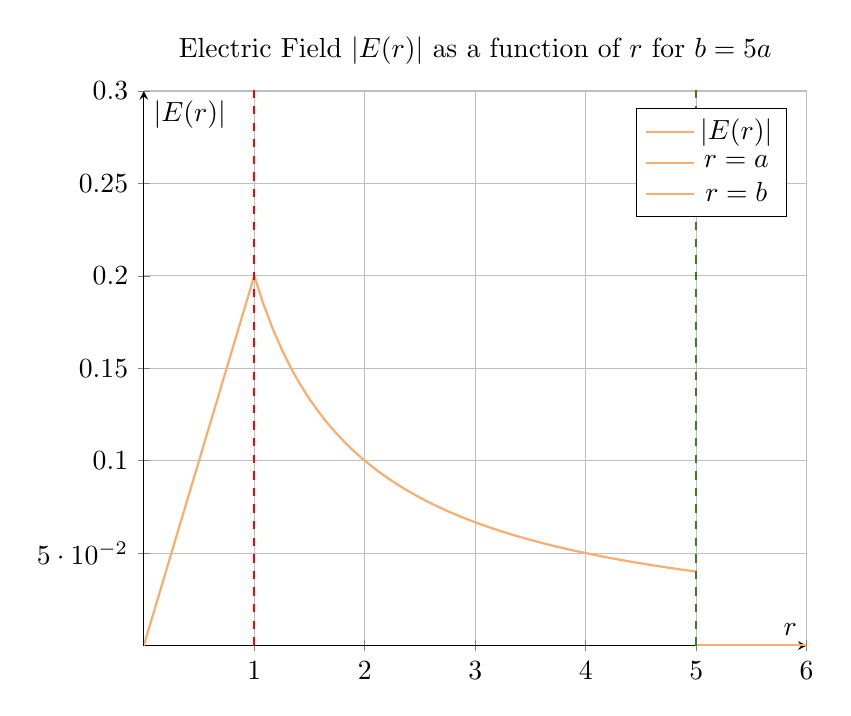
\begin{tikzpicture}
            \begin{axis}[
                    width=10cm,
                    xlabel={$r$},
                    ylabel={$|E(r)|$},
                    title={Electric Field $|E(r)|$ as a function of $r$ for $b = 5a$},
                    grid=major,
                    legend pos=north east,
                    axis lines=middle,
                    domain=0:6,
                    samples=200,
                    ymax=1.5,
                    xmin=0,
                    ymax=0.3
                ]

                % Region 1: E(r) = (rho * r) / (2 * epsilon_0) for r < a
                \addplot[domain=0:1, samples=50, thick, Apricot] {0.2*x};

                % Region 2: E(r) = (rho * a^2) / (2 * epsilon_0 * r) for a <= r <= b
                \addplot[domain=1:5, samples=50, thick, Apricot] {0.2*1^2/x};

                % Region 3: E(r) = 0 for r > b
                \addplot[domain=5:6, samples=50, thick, Apricot] {0};

                % Mark a and b
                \addplot[dashed, thick, red] coordinates {(1,0) (1,1)};
                \addplot[dashed, thick, OliveGreen] coordinates {(5,0) (5,1)};

                % Annotations for a and b
                \node at (axis cs:1,1.1) [anchor=south east] {$r = a$};
                \node at (axis cs:5,1.1) [anchor=south west] {$r = b$};

                \legend{$|E(r)|$, $r = a$, $r = b$}
            \end{axis}
        \end{tikzpicture}
    \end{figure}

    \end{homeworkProblem}

\newpage
\begin{homeworkProblem}
    Find the potential at a distance $z$ above a circular loop of radius $r$ that carries a uniform line charge $\lambda$. (NOTE: You can check this answer against the answer of Homework \#3 using $E = -\nabla V$.)
    \begin{callout}{Solution:}
        
        The electric field for a closed loop is given by:
        $$\frac{\lambda}{2 \epsilon_0} \frac{rz}{(r^2+z^2)^{3/2}}$$

        Integrate for the potential; first making a u-substitution $u=r^2 + z^2$
        \begin{align*}
            V(z) &= -\frac{\lambda r}{4 \epsilon_0} \int_{\infty}^{z} \frac{1}{(u)^{3/2}} ~du \\ 
            &= -\frac{\lambda r}{2 \epsilon_0} \left. \frac{1}{\sqrt{ r^2+z^2 }} \right|_{\infty}^{z} \\ 
            &= \frac{\lambda r}{2 \epsilon_0} \frac{1}{\sqrt{ r^2+z^2 }} 
        \end{align*}



    \end{callout}
\end{homeworkProblem}
